\documentclass{article}

\usepackage[margin=1in]{geometry}
\usepackage{amsmath}
\usepackage{graphicx}
\usepackage{multicol}
\usepackage{fancyvrb}

\begin{document}
	
\title{ESOF 422 - Homework 3}
\author{Nathan Stouffer and Kevin Browder}

\maketitle
\newpage

\section*{Question 1}
	For our FPS we are assuming the player can always see the player attacking and cannot be ambushed and attacked by a player out of view.  
	\begin{figure}[h]
		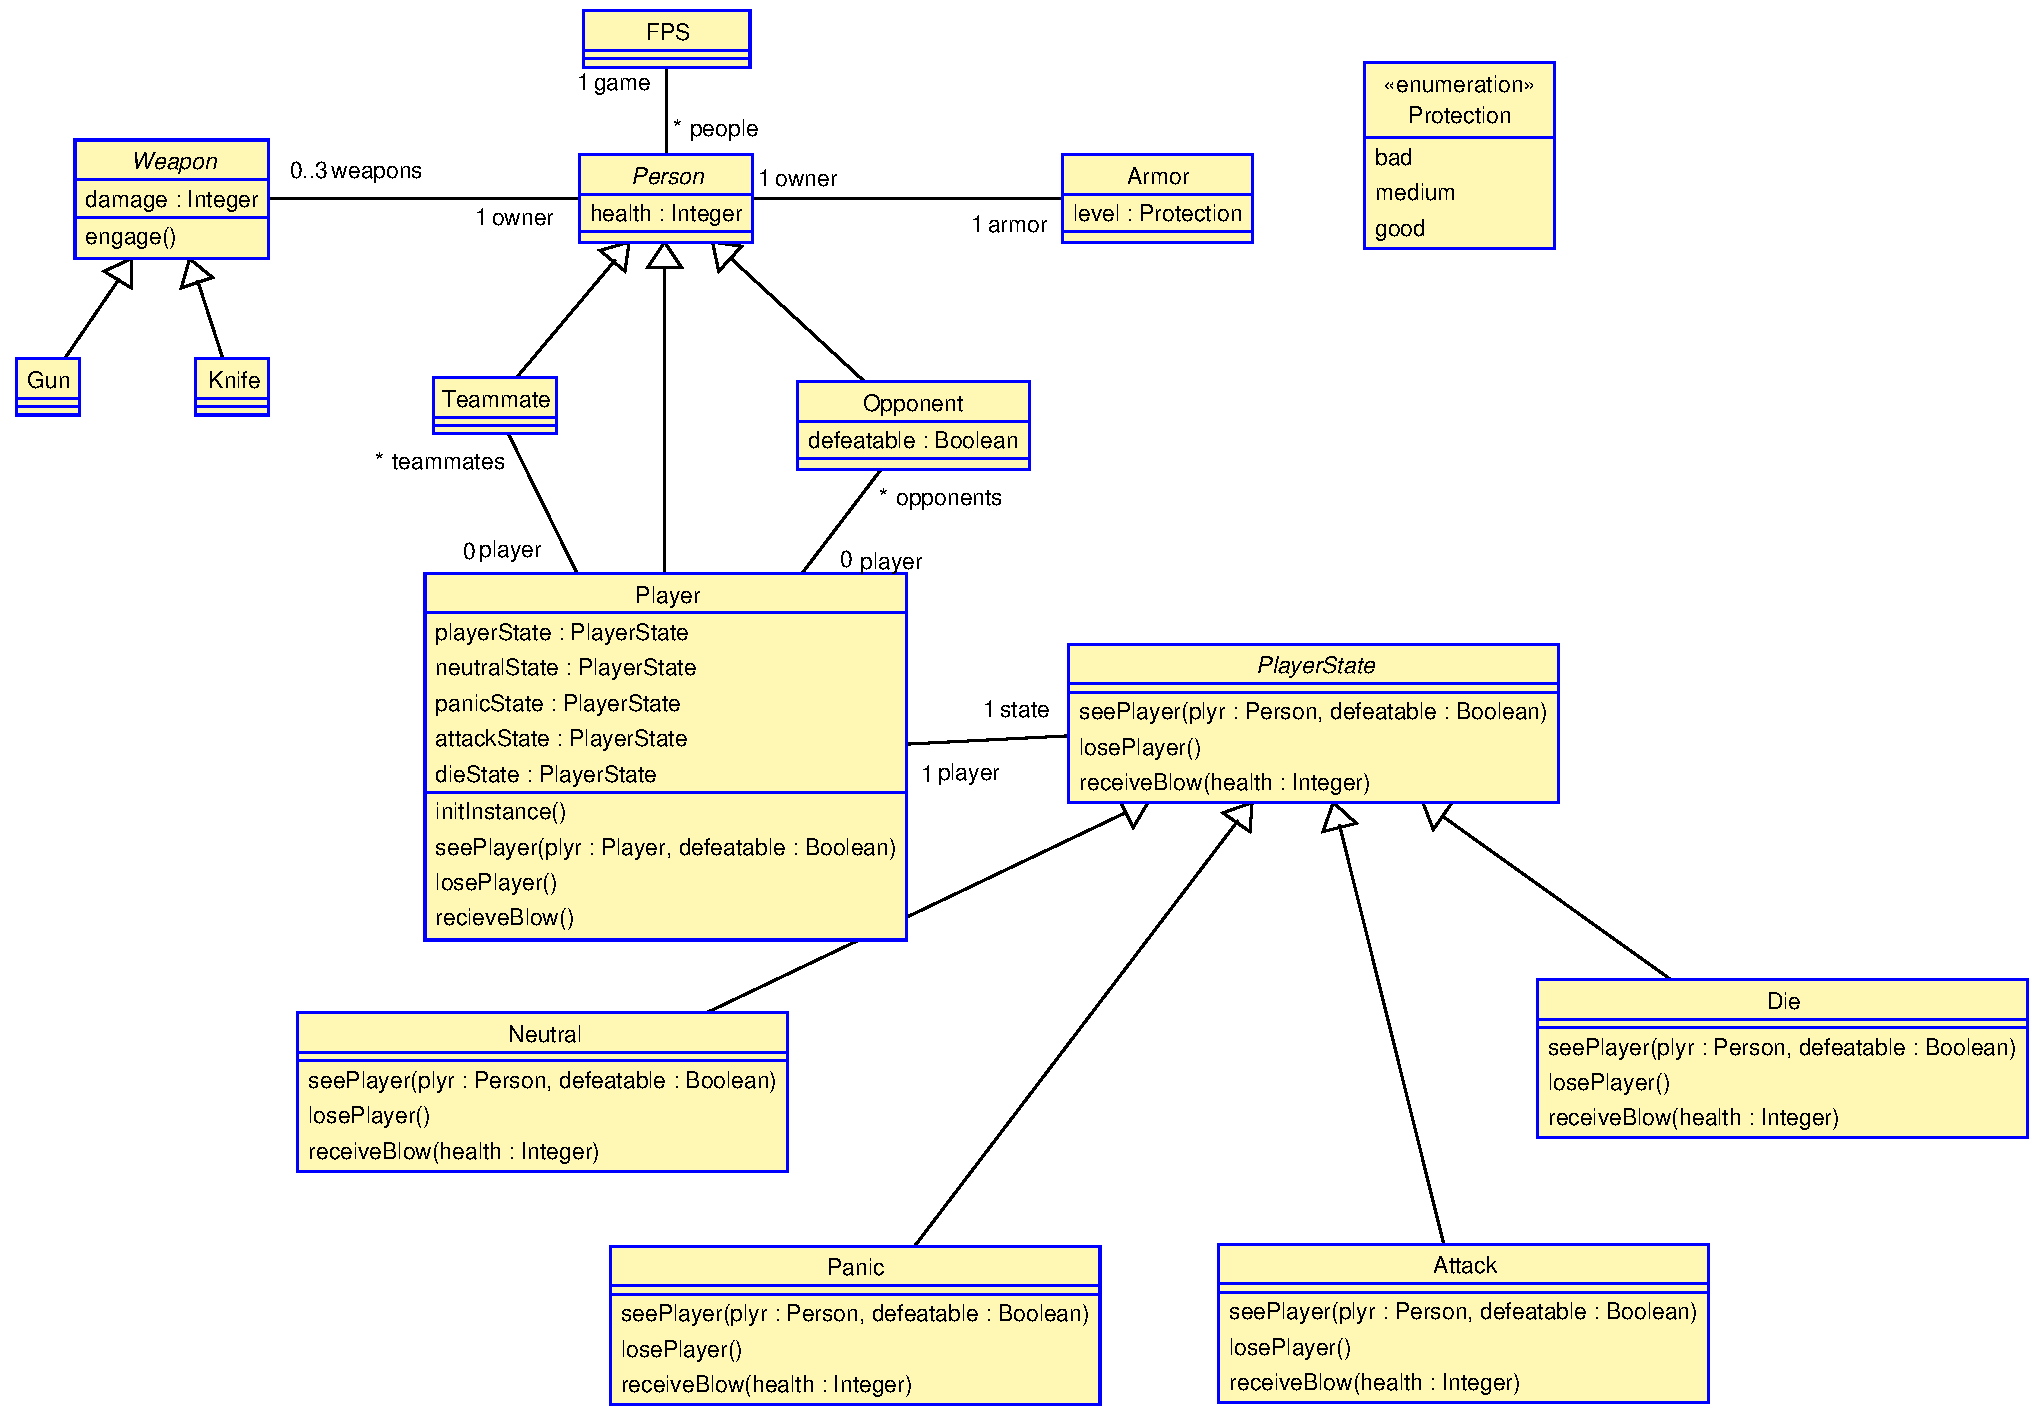
\includegraphics[width=\linewidth]{fps-class-diag.pdf}
		\caption{FPS Class Diagram}
		\label{fig:q1class}
	\end{figure}
	
	\begin{figure}[h]
		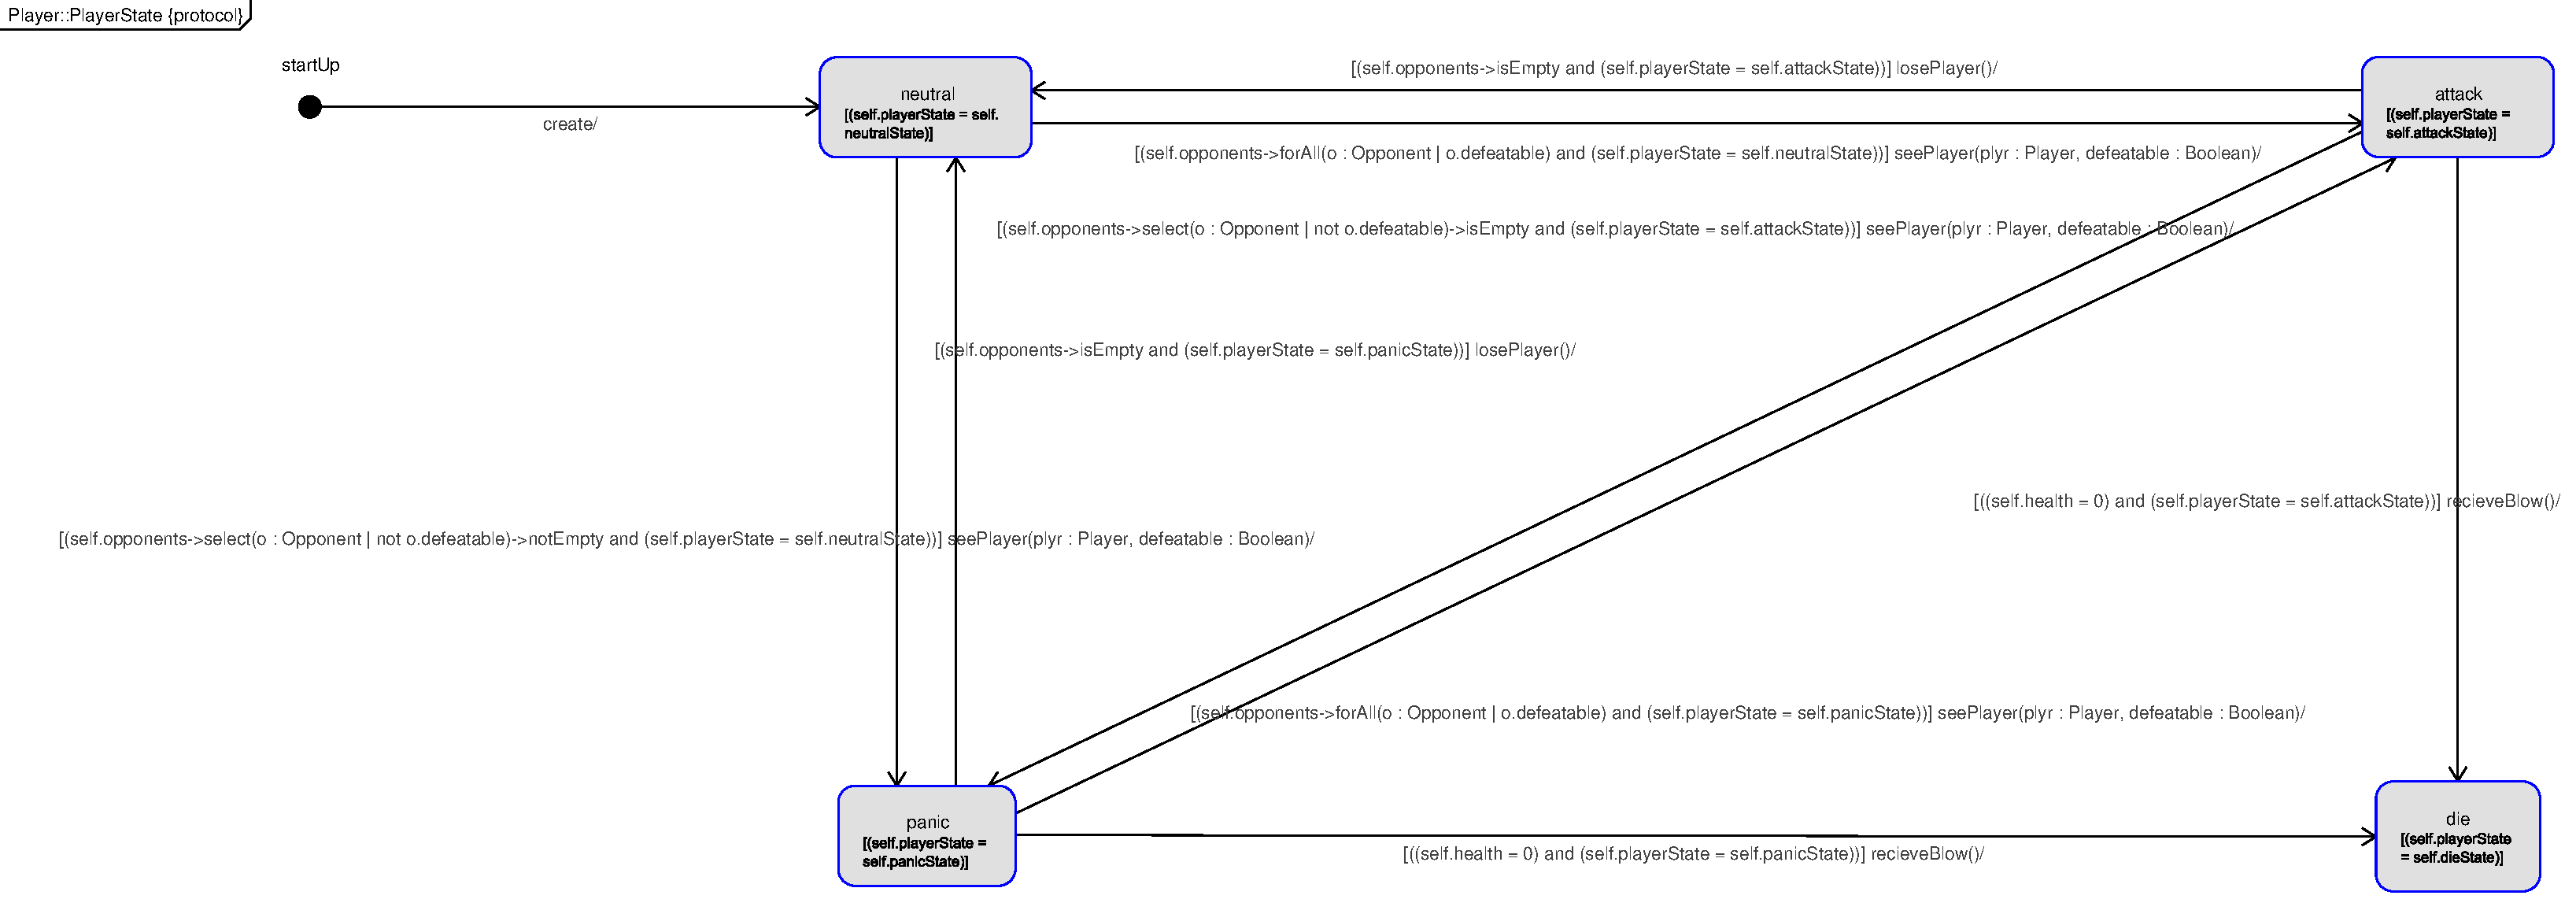
\includegraphics[width=\linewidth]{fps-state-diag.pdf}
		\caption{FPS State Diagram}
		\label{fig:q1class}
	\end{figure}
	\newpage
	
	.use Code
	
	\begin{Verbatim}
		/* This is a state machine model for a first person shooter game */
		
		model FPS
		
		-- enumerations
		
		-- define enumeration for protection level
		enum Protection {bad, medium, good}
		
		-- class definitions
		
		/* The following classes are an implementation of the state patter for a
		* player in this first person shooter
		*/
		
		abstract class PlayerState
		operations
		seePlayer(plyr: Person, defeatable: Boolean)
		begin
		end
		
		losePlayer()
		begin
		end
		
		receiveBlow(health: Integer)
		begin
		end
		end
		
		class Neutral < PlayerState
		operations
		seePlayer(plyr: Person, defeatable: Boolean)
		begin
		if (plyr.oclIsTypeOf(Teammate)) then
		WriteLine('In state:Neutral operation:seePlayer SEEN PLAYER IS A TEAMMATE');
		end;
		if (plyr.oclIsTypeOf(Opponent) and defeatable) then
		self.player.playerState := self.player.attackState;
		end;
		if (plyr.oclIsTypeOf(Opponent) and not defeatable) then
		self.player.playerState := self.player.panicState;
		end;
		end
		
		losePlayer()
		begin
		self.player.playerState := self.player.neutralState;
		end
		
		receiveBlow(health: Integer)
		begin
		if (health = 0) then
		self.player.playerState := self.player.dieState;
		end;
		end
		end
		
		class Panic < PlayerState
		operations
		seePlayer(plyr: Person, defeatable: Boolean)
		begin
		if (plyr.oclIsTypeOf(Teammate)) then
		WriteLine('In state:Panic operation:seePlayer SEEN PLAYER IS A TEAMMATE');
		end;
		if (plyr.oclIsTypeOf(Opponent) and not defeatable) then
		WriteLine('In state:Attack operation:seePlayer SEEN PLAYER IS AN OPPONENT - NO TRANSITION');
		end;
		if (plyr.oclIsTypeOf(Opponent) and defeatable) then
		self.player.playerState := self.player.attackState;
		end;
		end
		
		losePlayer()
		begin
		self.player.playerState := self.player.neutralState;
		end
		
		receiveBlow(health: Integer)
		begin
		if (health = 0) then
		self.player.playerState := self.player.dieState;
		end;
		end
		end
		
		class Attack < PlayerState
		operations
		seePlayer(plyr: Person, defeatable: Boolean)
		begin
		if (plyr.oclIsTypeOf(Teammate)) then
		WriteLine('In state:Attack operation:seePlayer SEEN PLAYER IS A TEAMMATE');
		end;
		if (plyr.oclIsTypeOf(Opponent) and not defeatable) then
		self.player.playerState := self.player.panicState;
		end;
		if (plyr.oclIsTypeOf(Opponent) and defeatable) then
		WriteLine('In state:Attack operation:seePlayer SEEN PLAYER IS AN OPPONENT - NO TRANSITION');
		end;
		end
		
		losePlayer()
		begin
		self.player.playerState := self.player.neutralState;
		end
		
		receiveBlow(health: Integer)
		begin
		if (health = 0) then
		self.player.playerState := self.player.dieState;
		end;
		end
		end
		
		class Die < PlayerState
		operations
		seePlayer(plyr: Person, defeatable: Boolean)
		begin
		WriteLine('In state:die  operation:seePlayer PLAYER CANNOT DO ANYTHING WHILE DEAD');
		end
		
		losePlayer()
		begin
		WriteLine('In state:die  operation:losePlayer PLAYER CANNOT DO ANYTHING WHILE DEAD');
		end
		
		receiveBlow(health: Integer)
		begin
		WriteLine('In state:die  operation:receiveBlow PLAYER CANNOT DO ANYTHING WHILE DEAD');
		end
		end
		
		class FPS
		attributes
		operations
		end
		
		abstract class Person
		attributes
		health: Integer init: 100
		operations
		end
		
		class Opponent < Person
		attributes
		defeatable: Boolean init: true
		operations
		end
		
		class Teammate < Person
		attributes
		operations
		end
		
		class Player < Person
		attributes
		playerState : PlayerState
		neutralState : PlayerState
		panicState : PlayerState
		attackState : PlayerState
		dieState : PlayerState
		
		operations
		initInstance()
		begin
		self.neutralState := new Neutral;
		self.panicState := new Panic;
		self.attackState := new Attack;
		self.dieState := new Die;
		
		self.playerState := self.neutralState; -- we start in neutral state
		end
		
		seePlayer(plyr: Player, defeatable: Boolean)
		begin
		self.playerState.seePlayer(plyr, defeatable);
		end
		
		losePlayer()
		begin
		
		end
		
		recieveBlow()
		begin
		
		end
		
		-- state machine for a Player
		
		statemachines
		
		/* The following state machine tracks the state of a player in
		* a first person shooter game */
		psm PlayerState
		states
		-- the start node
		startUp:initial
		neutral       [playerState = neutralState]
		panic         [playerState = panicState]
		attack        [playerState = attackState]
		die           [playerState = dieState]
		transitions
		-- define transition to initial state
		startUp -> neutral      { create }
		neutral -> panic { [opponents->select(o|not o.defeatable)->notEmpty and playerState = neutralState] seePlayer() }
		neutral -> attack { [opponents->forAll(o|o.defeatable) and playerState = neutralState] seePlayer() }
		panic -> attack { [opponents->forAll(o|o.defeatable) and playerState = panicState] seePlayer() }
		panic -> neutral { [opponents->isEmpty and playerState = panicState] losePlayer() }
		panic -> die { [health = 0 and playerState = panicState] recieveBlow() }
		attack -> neutral { [opponents->isEmpty and playerState = attackState] losePlayer() }
		attack -> panic { [opponents->select(o|not o.defeatable)->isEmpty and playerState = attackState] seePlayer() }
		attack -> die { [health = 0 and playerState = attackState] recieveBlow() }
		end
		end
		
		abstract class Weapon
		attributes
		damage: Integer
		operations
		engage()
		end
		
		class Knife < Weapon
		attributes
		operations
		end
		
		class Gun < Weapon
		attributes
		operations
		end
		
		class Armor
		attributes
		level: Protection
		operations
		end
		
		-- define associations
		
		association fps_people between
		FPS[1] role game
		Person[0..*] role people
		end
		
		association player_opponents between
		Player[0] role player
		Opponent[0..*] role opponents
		end
		
		association player_teammates between
		Player[0] role player
		Teammate[0..*] role teammates
		end
		
		association player_weapons between
		Person[1] role owner
		Weapon[0..3] role weapons
		end
		
		association player_armor between
		Person[1] role owner
		Armor[1] role armor
		end
		
		association player_playerState between
		Player[1] role player
		PlayerState[1] role state
		end
		
		-- define ocl constraints
		
		constraints
		
		context Person
		inv: health >= 0 and health <= 100
		
	\end{Verbatim}


\end{document}